
\par
Wszystkie elementy wyświetlające dane z pliku \DICOM dziedziczą po klasie \sokarclass{SceneIndicator}.
Diagram klas UML znajduje się na rysunku \ref{uml:sokar-scene-indicators}.

\begin{figure}[!htbp]
    \centering
    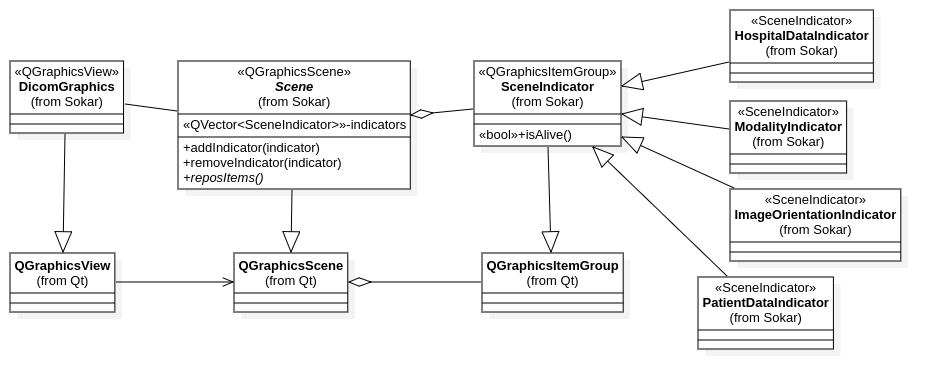
\includegraphics[width=\textwidth]{img/uml/dicom-scene-indicators.png}
    \caption{Diagram klas UML dziedziczenia klasy \sokarclass{SceneIndicator}.}
    \label{uml:sokar-scene-indicators}
\end{figure}

\par
Domyślnie obiekty wyświetlające informacje (tytuły punktów to nazwy klas):

\paragraph{Dane pacjenta}

Dane pacjenta są implementowane przez \sokarclass{PatientDataIndicator} i pojawiają się zawsze na scenie w lewym górnym rogu.
Zawierają następujące linie:
\begin{itemize}
    \item Nazwa pacjenta oraz płeć

          Nazwa pacjenta znajduje się w \dicomtag{Patient Name}{0010}{0010} o \dicomvr{PN}.

          Płeć, zapisana jest w \dicomtag{Patient Sex}{0010}{0040} i może mieć następujące wartości:
          \begin{itemize}
              \item \dataword{M } --- oznacza mężczyznę, wyświetlana jako znak \utfMaleSign
              \item \dataword{F } --- oznacza kobietę, wyświetlana jako znak \utfFemaleSign
              \item \dataword{O } --- oznacza inną płeć i nie jest wyświetlana
          \end{itemize}

          Przykład: \enquote{Jan Nowak \utfMaleSign}.

    \item Identyfikator pacjenta

          Unikalny identyfikator pacjenta ze znacznika \dicomtag{Patient ID}{0010}{0020} wyświetlany jest w takiej formie, w jakiej jest zapisany.
          W praktyce najczęściej jest to numer z systemu używanego w danym szpitalu, rzadziej numer PESEL.

          Przykład: \enquote{HIS/000000}.

    \item Data urodzenia oraz wiek pacjenta w trakcie badania

          Data urodzenia znajdująca się w \dicomtag{Patient Birth Date}{0010}{0030} i jest zamieniana na format \dataword{YYYY-MM-DD}.
          Dodatkowo, jeżeli tag \dicomtag{PatientAge}{0010}{1010} jest obecny, wyświetlany jest także wiek pacjenta w czasie badania.

          Przykład: \enquote{born 1982-08-09, 28 years}.

    \item Opis lub klasyfikacja badania dokonana przez instytucję

          Tekst brany z \dicomtag{Study Description}{0008}{1030} i wyświetlany bez ingerencji.

          UWAGA: Ta wartość jest wpisywana przez technika, operatora lub lekarza wykonującego badanie, więc wartość ta może być nieprzewidywalna.

    \item Opis serii

          Tekst brany z \dicomtag{Series Description}{0008}{103E} i wyświetlany bez ingerencji.

          UWAGA: Ta wartość jest wpisywana przez technika, operatora lub lekarza wykonującego badanie, więc wartość ta może być nieprzewidywalna.
\end{itemize}

Przykład pełnego teksu:

\begin{center}
    \begin{tabular}{l}
        \textbf{Jan Nowak} \utfMaleSign \\
        HIS/123456                              \\
        born 1996-01-01, 19 years               \\
        Kregoslup ledzwiowy a-p + boczne        \\
        AP
    \end{tabular}
\end{center}

\paragraph{Dane jednostki organizacyjnej}

Dane jednostki organizacyjnej są implementowane przez \sokarclass{HospitalDataIndicator}.
Pojawiają się zawsze na scenie w prawym górnym rogu i zawierają następujące linie:
\begin{itemize}
    \item Nazwa instytucji

          Tekst jest obierany z \dicomtag{Institutional Department Name}{0008}{1040} i wyświetlany bez ingerencji.

    \item Producent wyposażenia wraz z modelem urządzenia

          Tekst jest obierany z \dicomtag{Manufacturer}{0008}{0070} i \dicomtag{Manufacturer Model Name}{0008}{1070}, oddzielony spacją i wyświetlany bez ingerencji.

    \item Nazwisko lekarza wykonującego badanie

          Tekst jest obierany z \dicomtag{Referring Physician Name}{0008}{0090} i wyświetlany bez ingerencji.

    \item Nazwisko operatora wspierającego badanie

          Tekst jest obierany z \dicomtag{Operators Name}{0008}{1070} i wyświetlany bez ingerencji.
\end{itemize}

\paragraph{Orientacja obrazu}

\par
Orientacja obrazu jest implementowana przez \sokarclass{ImageOrientationIndicator}.
Obiekt wyświetla cztery litery oznaczające orientację obrazu w stosunku do pacjenta.
Obiekt posiada cztery pola: lewe, górne, prawe i dolne.

\par
Każda z sześciu możliwych liter oznacza kierunek oraz zwrot w jakim jest ułożony pacjent:
\begin{itemize}
    \item \enquote{R} --- right --- część prawa pacjenta
    \item \enquote{L} --- left --- część lewa pacjenta
    \item \enquote{A} --- anterior --- przód pacjenta
    \item \enquote{P} --- posterior --- tył pacjenta
    \item \enquote{F} --- feet --- część dolna pacjenta
    \item \enquote{H} --- head --- część górna pacjenta.
\end{itemize}

\par
Pełny opis implementacji algorytmu wyznaczania stron znajduje się w sekcji \ref{sec:algorithm-imageorientationindicator}.

\paragraph{Podziałka}

Podziałka Jest implementowana przez \sokarclass{PixelSpacingIndicator}.
Obiekt wyświetla podziałkę informującą o rzeczywistych rozmiarach obiektu na obrazie.
Pojawiają się na dole i po prawej stronie sceny, gdy znacznik \dicomtag{PixelSpacing}{0028}{0030} jest obecny.
Wygląd podziałki można zaobserwować na rysunku \ref{fig:imageorientationindicator1}.

Podziałka dostosowuje swoją wielkość do obecnej sceny, jak i do innych elementów na scenie.
Wartości wyświetlane biorą pod uwagę transformatę skali i rotacji obrazu.

\paragraph{Dodatkowe informacje o modalności}

Te informacje są implementowane przez \sokarclass{ModalityIndicator}.
Obiekt wyświetla informacje o akwizycji obrazu.
Dane różnią się w zależności od modalności obrazu.
Domyślnie zawierają następujące linie:
\begin{itemize}
    \item \enquote{Modality} --- modalność --- pobierana ze znacznika \dicomtag{Modality}{0008}{0060}.
    \item \enquote{Series} --- numer serii --- pobierany ze znacznika \dicomtag{Series Number}{0020}{0011}.
    \item \enquote{Instance number} --- numer instancji w serii --- pobierany ze znacznika \dicomtag{Instance Number}{0020}{0013}.
    \item Wartości odnoszące się do właściwości plastra obrazu.
          \enquote{Slice thickness} --- grubość plastra --- pobierana ze znacznika \dicomtag{Slice Thickness}{0018}{0050}.
          \enquote{Slice location} --- pozycja plastra --- pobierana ze znacznika \dicomtag{Slice Location}{0020}{1041}.
\end{itemize}

W przypadku następujących modalności zawierają również następujące informacje:
\begin{itemize}
    \item CT --- tomografia komputerowa
          \begin{itemize}
              \item \enquote{KVP} --- szczytowe napięcie wyjściowe generatora promieniowania rentgenowskiego --- wyrażone w kilovoltach, pobierane z \dicomtag{KVP}{0018}{0060}
              \item \enquote{Exposure time} --- czas ekspozycji --- pobierany ze znacznika \dicomtag{Exposure Time}{0018}{1150}.
              \item \enquote{Exposure} --- ekspozycja --- wyrażona w $mAs$, pobierana ze znacznika \dicomtag{Exposure}{0018}{1152}.
          \end{itemize}

    \item RT/CR --- radiologia analogowa i cyfrowa
          \begin{itemize}
              \item \enquote{Exposure time} --- czas ekspozycji --- pobierany ze znacznika \dicomtag{Exposure Time}{0018}{1150}.
              \item \enquote{KVP} --- szczytowe napięcie wyjściowe generatora promieniowania rentgenowskiego wyrażone w kilovoltach, pobierane z \dicomtag{KVP}{0018}{0060}
          \end{itemize}

    \item MR --- rezonans magnetyczny
          \begin{itemize}
              \item \enquote{Repetition time} --- czas repetycji --- pobierany ze znacznika \dicomtag{Repetition Time}{0018}{0080}.
              \item \enquote{Echo time} --- czas echa --- pobierany ze znacznika \dicomtag{Echo Time}{0018}{0081}.
              \item \enquote{Magnetic field} --- pole magnetyczne --- nominalna wartość pola magnetycznego wyrażona w teslach pobierana ze znacznika \dicomtag{Magnetic Field Strength}{0018}{0087}.
              \item \enquote{SAR} --- swoiste tempo pochłaniania energii --- pobierane ze znacznika \dicomtag{SAR}{0018}{1316}.
          \end{itemize}
\end{itemize}